El suelo ha sido objeto de estudios y análisis durante muchos años, ingenieros y científicos de gran relevancia en la ciencia han incursionado en los campos relacionados con la química y mecánica del suelo, proporcionando ideas y teorías fundamentales que han servido como base para construir desarrollo en temas concernientes a la capacidad de resistencia, límite de la capacidad estructural y pro elasticidad del suelo \parencite{field2011soil}. Áreas de conocimiento en mecánica del suelo que han sido claves para avanzar en el fortalecimiento de métodos de trabajo y factores de desempeño técnico que permiten desarrollar estrategias que mejoran la ejecución de proyectos, por ejemplo; la estabilidad en construcciones de edificaciones y obras, mejoramientos de cultivos y campos, etcétera.\\

Científicos como Henrry Darcy (1803 – 1858) y Robert Hooke  (1635 – 1703), aportaron grandes teorías que posteriormente se establecieron como leyes experimentales e indudables, las cuales fueron extremadamente dicientes al responder entre otras, una pregunta muy interesante \textit{¿cómo se mide un comportamiento entre un fluido y un medio poroso?}, Los hallazgos que obtuvieron experimentalmente estos científicos en busca de una respuesta originaron conceptos fundamentales en el estudio de la mecánica de suelos, como; ley de Darcy, ley de Hooke, ley de conservación de masas, concepto de deformación y tensión en medios deformables, poreslasticida entre muchos más \parencite{munozsimulacion}.  Estos conceptos asociados entre sí, permitieron conocer a fondo la estructura que forma la ciencia del suelo en toda su extensión, pues las ecuaciones matemáticas que conforman las leyes de Darcy, conservación de masas y Hooke, expresan de forma precisa que el alargamiento unitario que experimenta un material elástico es directamente proporcional a la fuerza aplicada sobre el mismo, así como también describen el comportamiento de líquidos a travez de medios porosos  \parencite{barrere1992closure}. Dejando así avances significativos en las áreas de mecánica y ciencia del suelo, permitiendo que se crearan nuevas fuentes de estudios en esas mismas disciplinas. El flujo del agua en el suelo está condicionado por muchas variables de tipo físico, entre algunas está la gravedad, la permeabilidad del suelo, la densidad, la humedad y la viscosidad del agua, por lo que para determinar el comportamiento de un fluido a través de un medio poroso como la arena no es tarea fácil, sin embargo es importante mencionar que muchos científicos e investigadores tratan de resolver las ecuaciones que permiten modelar dichos comportamientos característicos, pues con las interpretaciones y hallazgos que se consiguen se pueden determinar, por ejemplo, cual es la capacidad de agua disponible para un cultivo, cual es la capacidad de recarga de un acuífero, entre muchas mas aplicaciones.

\section{Modelos matemáticos con influencia en el agro}
%ley de  Poiseuille %

\subsection{\textbf{Ley de Poiseuille}}

\label{seccionleydePoiseuille}
 
En el estudio de física y mecánica de suelos a lo largo de cientos de años se han construido teorías, ideas y fundamentos que han permitido edificar sobre ellos construcciones que luego se convierten en leyes fundamentales que permiten el avance de todo tipo de aplicaciones en el suelo y referentes del mismo. Dichas teorías han sido tan importantes que aún en este tiempo se consideran temas principales a investigar pues permiten afianzar ideas para con esto estudiar otras leyes como la que se expone en la ley de Darcy (ver sección \ref{seccionleydeDarcy}). Siguiendo la idea anterior, la Ley de Poiseuille es una ley que permite calcular el flujo estacionario $\Phi_{V}$ de un líquido incompresible y viscoso también llamado \textbf{Fluido Newtoniano} a través de un tubo cilíndrico de sección circular en condición constante \parencite{PFITZNER1976}.\\

Según \parencite{PFITZNER1976} Cuando ocurren diferencias en el potencial hídrico del suelo, se produce un gradiente de potencial entre las regiones desde donde fluye mejor el agua hasta donde ocurre un menor flujo de la misma, haciendo relativamente sencillo el cálculo de la dirección del flujo de agua del suelo en cualquier situación. Sin embargo si se necesita conocer la relación entre las diferencias de potencial hídrico y la tasa de flujo, se debe considerar la ley de Poiseuille para el flujo laminar a través de un tubo la cual se expresa como:

\begin{equation}
	\label{ecuaciondepoiseuille}
	\varrho=\frac{\pi r^{4}}{8 \eta} \frac{\Delta p}{L}
\end{equation} 

Siendo en la ecuación \eqref{ecuaciondepoiseuille} $Q$ el volumen de flujo por unidad de tiempo $\left(\mathrm{m}^{3} \mathrm{~s}^{-1}\right), r$ es el radio del tubo $(\mathrm{m}), \Delta$ p es la diferencia de presión de un extremo del tubo al otro $(\mathrm{Pa}), \eta$ es la viscosidad dinámica del fluido $(\mathrm{Pa} \times \mathrm{s})$, y $\mathrm{L}$ es la longitud del tubo $(\mathrm{m})$. Es importante tener en cuenta que el término $\frac{\Delta p}{L}$ es una equivalencia a la diferencia del potencial hídrico de un punto del suelo a otro. Es entonces que $\frac{\Delta p}{L}$ define al gradiente hidráulico.\\

La ley de Poiseuille permite considerar no solo el caudal volumétrico $\mathrm{Q}$, sino también el flujo $\mathrm{q}$ tomándolo como caudal volumétrico por unidad de área $\left(\mathrm{ms}^{-1}\right)$. Al considerar que el área de la sección transversal de un tubo cilíndrico es $\pi r^{2}$, el flujo a través de un tubo está dado por:

\begin{equation}
	\label{2ecuaciondepoiseuille}
	q=\frac{r^{2}}{8 \eta} \frac{\Delta p}{L}
\end{equation}

Observando que en la ecuación \eqref{2ecuaciondepoiseuille} $r^2$ muestra la magnitud del flujo para un gradiente hidráulico particular pues esta depende del radio del tubo. Este principio se puede concretizar al flujo del agua en el suelo,  pues el flujo de agua a través del suelo depende en gran medida del tamaño de los poros del mismo.\\

Las viscosidades del agua y el aire, los dos fluidos que encuentran con mayor frecuencia en el suelo, aumentan a medida que desciende la temperatura. Por lo tanto, a partir de la ley de Poiseuille, se puede inferir que las tasas de flujo de estos fluidos a través del suelo disminuirán a medida que disminuya la temperatura.\\


La ecuación de Poiseuille ha sido útil y aplicable en muchos sistemas naturales e industriales, tanto en sistemas biológicos como por ejemplo, vasos sanguíneos y huesos, también en la hidrología y en los suelos. Es así que \parencite{Eberhard2019} 
en su investigación reconoce, que aunque en la gran mayoría de fluidos newtonianos que fluyen a través de un medio poroso la fórmula mas recurrente a utilizar es la ley de Darcy \eqref{Darcyeq1}, sin embargo la relación entre la caída de presión y velocidad de un fluido en la ecuación de Darcy no están bien definidas  pues no pueden describirse mediante una función lineal como es el caso de los fluidos newtonianos. Por tanto \parencite{Eberhard2019} no excluyó la  implementación de la ecuación de Poiseuille para dar una globalización para la formulación de solución al flujo lineal en la caída de presión, utilizando la viscosidad que a su vez depende de variables de flujo.\\

También \parencite{Xenakis2015} menciona que la ecuación y los flujos de Poiseuille son utilizados en su mayoría para la validación de métodos computacionales, puesto que las soluciones analíticas de estado estacionario son fácilmente expresadas como:

\begin{equation}
	\label{3ecuaciondePoiseuille}
	\frac{\partial u}{\partial t}=\frac{\partial \tau_{y x}}{\partial x}+F_{x}
\end{equation}

donde se describe de la ecuación \eqref{3ecuaciondePoiseuille} que $T$ Y $F_{x}$ son la velocidad y la fuerza del cuerpo en la dirección $x$ respectivamente, y  $\tau_{v m}=\mu_{\mathrm{aff}} \partial u / \partial y$ ya que $\partial v / \partial x=0$ para este caso. \\

También es importante como \parencite{Xenakis2015} realizó una admirable investigación acerca de la aplicación del método numérico derivado del lagrangiano llamado SPH, el cual ha sido aplicado desde los años 70s como una estrategia de modelamiento de fluidos incompresibles tratándolos como "débilmente compresibles". Para el desarrollo de soluciones y modelos matemáticos son consideradas complejas ecuaciones y técnicas estándar del cálculo de la viscosidad de fluidos, todas relacionadas con el flujo y presiones tensoriales ejercidas por un líquido sobre una superficie libre. En la metodología empleada por los investigadores se deja ver como al ellos relacionar y de alguna manera unir los conceptos de modelos matemáticos orientados a modelación de un flujo de un fluido en una superficie libre como por ejemplo; gradiente y divergencia, concepto de viscosidad, ecuación de Poisson enfocada a la presión y la ecuación de flujos de Poiseuille, Desarrollan un algoritmo de solución basado en la ampliación del método SPH, el cual permite resolver y modelar lo flujos in-elásticos no newtonianos. Se hace saber también que se realizó una validación computacional del método para asegurar su comprobación.   



%% ---ley de darcy---%%


\subsection{\textbf{Ley de Darcy}}

\label{seccionleydeDarcy}

Como ya se mencionó, Henry Darcy fue uno de los científicos que en su tiempo se interesó por la descripción y el flujo de un líquido como el agua a través de un medio poroso como la arena. La experiencia cotidiana nos dice que el agua puede viajar a través de la arena, pero la mayoría de las personas se conforman con este hecho únicamente en términos cualitativos, pocas personas se preguntan cómo se puede describir dicho flujo de forma cuantitativa, Darcy diseñó un experimento basado en ecuaciones diferenciales para calcular el caudal del agua en función de otros parámetros físicos, el cual se expresa así; 
\begin{equation}
	\Vec{q}=-K\frac{\varDelta{h}}{\varDelta{l}}
	\label{Darcyeq1}
\end{equation}

en donde se identifican; 

$k$ = conductividad hidráulica.

$\Vec{q}$ = caudal que circula por metro 
cuadrado de una sección.

$\frac{\varDelta{h}}{\varDelta{l}} \rightleftharpoons \frac{dh}{dl}$ = gradiente hidráulico expresado en incrementos infinitesimales.\\


Como se muestra en  la ecuación \eqref{Darcyeq1} Su hallazgo experimental es una ley importante y reconocida utilizándose hasta hoy en día para relacionar linealmente las diferencias entre presión y caudal de agua.\parencite{schweizer2015darcy}. De forma general la ley de darcy es una fórmula que describe como se mueve el agua a través de un medio poroso como el suelo, calculando de forma aproximada cuál es la velocidad que tiene el fluido teniendo en cuenta variables cuantificables experimentalmente como \textit{coeficiente de gradiente hidráulico,} \textit{conductividad hidráulica} o coeficiente de permeabilidad \parencite{rozas2002permeabilidad}.

\begin{figure}[h]
	\centering
	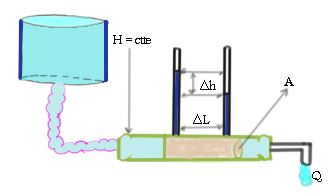
\includegraphics[scale=1]{Imagenes/Ley de Darcy 01.JPG}
	\caption{Experimento Permeámetro de carga constante de  Henry Darcy}
	\label{Darcy01}
\end{figure}

En la figura \ref{Darcy01} Henry Darcy descubrió este principio de velocidad de un fluido a través de un medio poroso por medio de un experimento que, como se intuye también puede ser replicado obteniendo datos aproximados de qué velocidad alcanza el fluido, teniendo en cuenta para este experimento también una variable $A$, la cual es el tamaño del cilindro donde se deposita el material poroso, en este caso arena \parencite{del1993flujo}, es decir  la ley de Darcy  indica que el caudal de agua $Q$ que se mueve a través de un determinado medio poroso es directamente proporcional a la sección transversal atravesada $A$ y al gradiente hidráulico $I$:
\begin{equation}
	Q = i*A
\end{equation}
Siendo $i$ el gradiente hidráulico que, como se observa en la imagen \ref{Darcy01}, se deduce realizando el cociente entre $\frac{\bigtriangleup h}{\bigtriangleup l}$, tendiendo en cuenta que $\bigtriangleup h$ es la diferencia de potencial entre una altura y otra correspondiente, así también  $\bigtriangleup l$ es el total de los estratos o la longitud de volumen cilíndrico a analizar, siendo la ecuación de Darcy expresada así;
\begin{equation}
	Q = -K* A (\frac{dh}{dl})
	\label{Darcyequ9}
\end{equation}

El signo menos de $K$ se debe a que el nivel disminuye en el sentido del flujo; es decir, que $\varDelta{h}$ o $\varDelta{l}$ son negativos y el signo menos hace que el caudal sea positivo. \\

La conductividad hidráulica,  tiene dos casos especiales donde se debe analizar su correcta aplicación en la fórmula de Darcy, cuando el flujo es paralelo a la capa a de suelo a analizar,  cuando el flujo es perpendicular a la capa de suelo a analizar, siguiendo el caso que corresponda la conductividad hidráulica identificada como $k$ tiene cambios en su estructura de ecuación, pues al tener que adaptarse a los cambios del fluido del suelo debe ampliar su operatividad incluyendo variables adaptativas de la matriz del suelo \parencite{hurtado2001succion}. Realizando un producto de variables y siguiendo el concepto de la ley de Darcy se puede obtener entonces la ecuación \ref{Darcyeq1}  Es valido también hacer mención del concepto de conductividad hidráulica, trata básicamente, y de forma general, en la facilidad con la que un medio poroso permite que el paso de un fluido a través de sus películas porosas sea rápido o lento, claro está que también tiene en cuenta variables ajenas a ella como la viscosidad del agua.\\ 

La ley de Darcy por su estructura y aplicabilidad tiene limitantes, en su artículo \parencite{romana2014limites} permite conocer que en la ecuación de Darcy la constante de proporcionalidad o conductividad hidráulica no es propia ni depende únicamente de un medio poroso, también depende de variables del fluido como la viscosidad entre otros. Por tanto solo se puede emplear en un medio saturado, continuo, homogéneo e isotrópico. De igual manera la ley de Darcy es plausible cuando se considera el flujo de agua subterránea, donde la viscosidad es prácticamente constante, ya que su valor casi no se ve afectado en vista de las pocas diferencias de temperatura a lo largo de una matriz de suelo. \\

Teniendo en cuenta lo anterior, la ley de Darcy también tiene muchas aplicaciones, pues es importante para predecir el flujo de agua a lo largo de un acuífero antes de efectuar la perforación de los pozos, también es usada regularmente en la ingeniería agrícola, ingeniería hidrológica y en la industria petrolera para describir el flujo de gas y petróleo en medios porosos. También \parencite{ruizmodelo} en su investigación hace saber que por medio de  modelos sistematizados se pueden realizar  aproximaciones fenomenológicamente del flujo de partículas en medios porosos y, que con un análisis estadístico se logra de forma aproximada simular los mecanismos  e impacto sobre la capacidad de flujo de una roca productora de hidrocarburos. Claro está que en su artículo se muestra la aplicabilidad que tiene la ley de Darcy pues la emplea para plantear y resolver ecuaciónes que le permiten, por ejemplo, determinar el flujo de varias fases en un medio poroso, obteniendo con la interacción de la Ley de Darcy la ecuación de flujo bifásico – líquido-partícula - en un medio poroso.\\

Como ya se mencionó, muchos investigadores han desarrollado contribuciones importantes para dar solución numérica a modelos matemáticos que en su estructuras se conforman por ecuaciones diferenciales parciales y que se enfocan en el movimiento característico de un fluido en un medio poroso saturado o no saturado. Entre los métodos numéricos más conocidos para solución de ecuaciones diferenciales parciales se encuentran diferencias finitas, volúmenes finitos, elementos de frontera, front tracking, Galerkin discontinuo, entre otros. Es interesante como \parencite{bastidasmetodo} en su tesis  da a conocer que el  método Galerkin Discontinuo es implementado para dar una solución a  la ecuación de Darcy. demostrando que el  estudio de esta ecuación clásica empleada mayormente en la mecánica de fluidos permite el análisis más básico de la interacción de un fluido con el medio y es ampliamente utilizada para avanzar en modelos más robustos como las ecuaciones de Stokes-Darcy o Navier-Stokes . \\


 

%% -----fin de ley de Darcy----%%

\section{Algunas varicaciones de la ley de Darcy}
% ---- Variaciones de la ley de Darcy----%

\subsection{Variaciones de la ley de Darcy}

Al pasar los años y desarrollarse nuevas tecnologías se han generado también diferentes situaciones y problemas a resolver. Es por eso que la ley de Darcy ha sido modificada a conveniencia por científicos e investigadores en aras de acercarse a un esquema de soluciones que permita avanzar en la resolución de problemas del agro y temas relacionados. Ingenieros y empíricos  de diferentes épocas se ha enfocado en unir conceptos, leyes y teoremas que han dado forma a diferentes variaciones de la ley de Darcy las cuales amplían de cierta manera el alcance de las ecuaciones desarrolladas permitiendo incluir en su estructura variables que relacionan medios porosos robustos entre otras. A continuación algunos ejemplos de lo anterior.

\subsubsection{Ecuación de Darcy-Weisbach}


Ésta ecuación es frecuentemente empleada en la dinámica de fluidos, dicha ecuación es totalmente empírica y relaciona la pérdida de carga hidráulica por la fricción a lo largo de una tubería teniendo en cuenta la velocidad de flujo del fluido. Contiene también un factor adimensional, conocido como factor de fricción de Darcy \parencite{Farras2000},\parencite{Manning1991}. Por tanto en la dinámica de fluidos es sabido que la ecuación de Darcy-Weisbach es fenomenológica, por tanto al relacionar la pérdida de carga principal en un espacio tubular debido a la fricción del flujo se puede considerar válida para un flujo monofásico y totalmente desarrollado, constante e incompresible.\\

La ecuación de Darcy-Weisbach se denota de maneras equivalentes. Una de las más comunes es la llamada \textbf{Forma de pérdida de cabeza.}, la cual se muestra a continuación.

\begin{equation}
	\frac{\Delta h}{L}=f_{\mathrm{D}} \cdot \frac{1}{2 g} \cdot \frac{V^{2}}{D}
	\label{forma de perdida de cabeza ecuacion de Darcy-weisbach}
\end{equation}

donde:\\

\noindent- $\Delta h$ = la pérdida de carga debido a la fricción (m).\\
- $f_{D}=$ el factor de fricción de Darcy (sin unidades).\\
- $L=$ la longitud del tubo $(m)$.\\
- $\mathrm{D}=$ el diámetro hidráulico de la tubería $\mathrm{D}(\mathrm{m}).$\\
- $g$ = la constante gravitacional $\left(\mathrm{m} / \mathrm{s}^{2}\right).$\\
- $V$ = la velocidad media del flujo $V(\mathrm{~m} / \mathrm{s}).$


Es importante mencionar que la ecuación \ref{forma de perdida de cabeza ecuacion de Darcy-weisbach} proporciona mucha información referentes a factores que afectan una pérdida considerable de carga en una tubería. Claro está que en el resultado de las evaluaciones a tuberías que se realicen  siempre se deben considerar mínimo una de las siguientes apreciaciones.

\begin{itemize}
	\item La longitud de la tubería o el canal se duplica, la pérdida de carga por fricción resultante se duplicará .
	\item A una velocidad de flujo constante y longitud de la tubería, la pérdida de carga es inversamente proporcional a la cuarta potencia de diámetro (para flujo laminar), y así reducir el diámetro de la tubería a la mitad aumenta la pérdida de carga en un factor de 16. Este es un aumento muy significativo. en pérdida de carga, y muestra por qué las tuberías de mayor diámetro conducen a requisitos de potencia de bombeo mucho más pequeños.
	\item Dado que la pérdida de carga es aproximadamente proporcional al cuadrado del caudal, entonces, si el caudal se duplica, la pérdida de carga aumenta en un factor de cuatro.
	\item La pérdida de carga se reduce a la mitad (para flujo laminar) cuando la viscosidad del fluido se reduce a la mitad.
\end{itemize}

Por otra parte, es preciso tener en cuenta que una diferencia de la ecuación de \textbf{Darcy-Weisbach} con la ley de Darcy es que ésta última emplea muchos más factores que involucran la tubería propiamente como el \textbf{Factor de fricción de Darcy}, por tanto dicho factor tiene en cuenta las propiedades de densidad y viscosidad del fluído junto con la rigurosidad de la tubería.

\subsubsection{ley de Darcy-Buckingham}

Una ley fundamental para tratar suelos no saturados es la ley \textbf{Darcy-Buckingham}, Pues al tratarse de suelos donde existen fluidos entre los poros como agua y aire la ley de Darcy presenta una pequeña modificación. Las burbujas de aire causan perturbaciones en los poros en que se encuentran el paso del líquido cuando este está permeante. así lo plantea en su tesis \parencite{Friaspineda2018} describiendo el porqué el grado de saturación del suelo va aumentando a  medida que aumentan las burbujas en medio de los poros. También, él menciona que el coeficiente de permeabilidad de los suelos parcialmente saturados aumenta en función de la presión del líquido. Es entonces que la ecuación toma la siguiente forma para suelos saturados.

\begin{equation}
	-K(\Psi)\left(\frac{\partial \Psi}{\partial z}+1\right)
	\label{ecuacion darcy-Buckinham}
\end{equation}

Siendo en la ecuación \eqref{ecuacion darcy-Buckinham} $z$ la coordenada vertical positiva hacia arriba, el potencial capilar del suelo $-K(\Psi)$, asimismo se tiene en cuenta que la función $-K(\Psi)$ permite resolverse para el flujo laminar del suelo.



%%---- Ecuación de Richard-----%%

\subsection{Ecuación de Darcy-Richards}

Existen ecuaciones diferenciales que se relacionan y complementan entre sí, en un contexto del movimiento de un fluido en un medio poroso. La ecuación de Richard por ejemplo es un modelo matemático fiable y más flexible que la ecuación de Darcy en su  operatividad, pues Richard propuso una ecuación diferencial parcial (EDP) no lineal basándose en una combinación de la ley de Darcy y la ecuación de continuidad, esta se expresa así; 

\begin{equation}
	\frac{\partial\theta}{\partial t}=\frac{\partial}{\partial z}(k(\psi)(\frac{\partial\psi}{\partial z}+1))
	\label{eq2}
\end{equation}

Como se puede observar en la ecuación \eqref{eq2} definiendo parámetros se permite describir el flujo de un líquido en un medio no saturado, pues la ley de Darcy inicialmente se fabricó para tratar flujos de líquidos en medios  saturados \parencite{mawloodcomparison}. El movimiento del agua en el suelo ocurre en principio en medios saturados y no saturados, la diferencia entre ellos radica en que en los suelos no saturados los espacios que hay entre los poros de una matriz de suelo son más pronunciados permitiendo que se almacene aire entre ellos,  por lo que es  fácil que un fluido como el agua se mueva de forma libre entre los poros del suelo, teniendo en cuenta lo anterior es más provechoso que un suelo tenga una condición de no saturación pues al retener más humedad el suelo y no estar completamente saturado el agua se mueve despacio laminarmente generando niveles óptimos de componentes matriciales en el suelo, generando entre muchos beneficios condiciones para un buen aprovechamiento en cultivos  \parencite{hernandez2012estimacion}.   También se tiene en cuenta que la ecuación de Richard carece de una solución general de forma cerrada, por lo que muchos investigadores han derivado modelos numéricos y analíticos para resolver la ecuación de Richard\parencite{perau1998constitutive}.\\

También es interesante conocer que  La ecuación de Richards es una expresión elíptica parabólica no lineal la cual permite estimar la conductividad hidráulica en el suelo no saturado, de acuerdo con  \parencite{luna2005metodos} esto es importante  porque la conductividad hidráulica es variable respecto al contenido de humedad que esta contenga, es decir; a medida que el agua se infiltra en el perfil del suelo el fluido que se mide es más cercano a la conductividad hidráulica medida experimentalmente, esto en el caso del suelo no saturado. Para el suelo con saturación la conductividad hidráulica es una variable que es representada por un valor único que se determina en condiciones de saturación máxima del suelo
La ecuación de Richards se basa en otras ecuaciones fundamentales para la ciencia del suelo, como lo es la ecuación de continuidad que dicho de forma general se emplea para saber cuanta agua está fluyendo por un volumen de suelo. Siguiendo de forma apreciativa a \parencite{martinez2013aproximacion} que en su tesis explica de forma muy general, como al unir la ecuación de Darcy y la ecuación de continuidad, se obtiene una equivalencia de la ecuación de Rirachds, análogamente se replicará el procedimiento pero claro está que no de forma teórica sino mejor de manera intuitiva.\\ 
\begin{figure}[h]
	\centering
	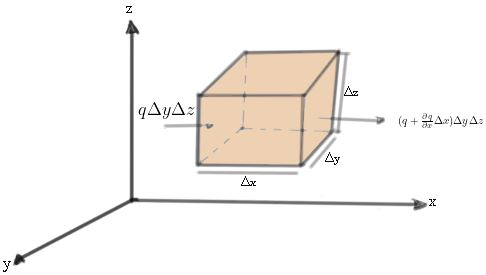
\includegraphics[scale=0.7]{Imagenes/Solido en 3D.JPG}
	\caption{Volumen de sólido en 3D}
	\label{richardseq1}
\end{figure}

En la figura \ref{richardseq1} se hace referencia a que el cubo es una porción de suelo o un volumen definido de suelo, el flujo de agua que entra por el eje de las coordenadas $x$ es expresado por la ecuación.

\begin{equation}
	q_{entra}= q_{x} \varDelta_{y}\varDelta_{z}
	\label{Richardseq2}
\end{equation}

Y el flujo que sale expresado en componentes espaciales en $x$, $y$ y $z$ está expresada así.
\begin{equation}
	q_{sale}=(q+ \frac{dq}{dx}\varDelta_{x})\varDelta_{y}\varDelta_{z}
	\label{Richardseq3}
\end{equation}
Estas expresiones lo que esencialmente están diciendo es que en un volumen de suelo representativo la humedad se gana o pierde según la divergencia del flujo en ese volumen, entendiéndose por divergencia a la cantidad de flujo que entra al volumen de suelo respecto a la cantidad que sale del mismo.\\


Calculando  \textbf{la tasa de flujo neta} $Tn$, restando la ecuación \eqref{Richardseq2} - la ecuación \eqref{Richardseq3} se obtiene lo siguiente.
$$ Tn = q_{x} \varDelta_{y}\varDelta_{z} - (q_{x}+ \frac{dq}{dx}\varDelta_{x})\varDelta_{y}\varDelta_{z}$$
Observando la ecuación se deduce que al aplicar la propiedad distributiva en la ecuación \eqref{Richardseq3} con los $\varDelta_{x}\varDelta_{y}\varDelta_{z}$ se cancelan los términos semejantes que tienen signos contrarios quedando lo siguiente.

\begin{equation}
	tn = - \frac{\partial q_{x}}{\partial x } \varDelta_{x}\varDelta_{y}\varDelta_{z}
	\label{Richardeq4}
\end{equation}

Teniendo en cuenta que el volumen que se analiza siempre tendrá un contenido de humedad que estará expresado con respecto al tiempo y no en coordenadas espaciales, es decir; el cambio del contenido de humedad o $tH$ está expresado no en el espacio sino con respecto al tiempo así:

\begin{equation}
	tH = \frac{\partial \theta}{\partial t} \varDelta_{x}\varDelta_{y}\varDelta_{z}
	\label{Richardeq5}
\end{equation}

Si el cambio del contenido de humedad es igual a la tasa de flujo entonces al igualar las ecuaciones \textit{Tasa de flujo neta} \eqref{Richardeq4} y \textit{tasa de cambio de Humedad} \eqref{Richardeq5} obtenemos:
$$- \frac{\partial q_{x}}{\partial x } \varDelta_{x}\varDelta_{y}\varDelta_{z} =  \frac{\partial \theta}{\partial t} \varDelta_{x}\varDelta_{y}\varDelta_{z}$$
Al notar que los componentes diferenciales $\varDelta_{x}\varDelta_{y}\varDelta_{z}$ en cada lado de la igualdad están multiplicando se pueden cancelar por operaciones elementales obteniendo entonces: 

$$ \frac{\partial \theta}{\partial t} = - \frac{\partial q_{x}}{\partial x }$$ en el eje de la coordenada $x$, en sí esta es la \textbf{ecuación de la continuidad} que dicta que el cambio en el contenido de humedad  es igual a la divergencia del flujo en el volumen de análisis.\\
Para poder tener en cuenta la ecuación en 3 dimensiones hay que observar el flujo en los 3 componentes espaciales así; 

\begin{equation}
	\frac{\partial \theta}{\partial t} = - (\frac{\partial q_{x}}{\partial x} + \frac{\partial q_{y}}{\partial y} + \frac{\partial q_{z}}{\partial z} )
	\label{Richardseq6}
\end{equation}\\
Se puede deducir la ecuación de Richard realizando la sustitución de la ley de Darcy \eqref{Darcyeq1} en la ecuación de la continuidad \eqref{Richardseq6} se puede obtener una equivalente a la ecuación de Richard, la cual es la ecuación general del flujo del agua en los suelos o medios porosos.
\begin{equation}
	\frac{\partial \theta}{\partial t} = - \frac{\partial}{\partial x}(k \frac{\partial \Phi}{\partial x}) \rightleftharpoons \frac{\partial \theta}{\partial t} = -k \frac{\partial^{2}h}{\partial^{2}x}
	\label{Richardseq7}
\end{equation}

Hay que tener en cuenta que $\frac{\partial \Phi}{\partial x}$ se entiende también como el gradiente hidráulico en la ley de darcy, se observa también en la ecuación \eqref{Richardseq7} que al ser una derivada de otra derivada se deduce que es una ecuación diferencial parcial  de segundo orden.     
De acuerdo con \parencite{CHAVEZNEGRETE2018168}  esta ecuación es muy importante para las ingenierías agrícolas e hidrológicas, por esto se han propuesto varios esquemas de linealización para aproximar su solución.  Se han propuesto combinaciones de iteraciones newtonianas para la discretización espacial  mediante diferencias, y un método  implícito para la integración temporal. Sin embargo, cuando se utiliza la formulación de diferencias finitas, se presentan oscilaciones numéricas cerca del frente de infiltración.\\

De acuerdo con \parencite{garza2013ecuaciones}, el éxito de las ecuaciones diferenciales parciales se concentra en su capacidad de modelar una enorme diversidad de fenómenos físicos, biológicos, químicos, de la ingeniería, de la economía, etcétera. Debido a la complejidad que implica el modelamiento de un fenómeno natural, Existen diferentes métodos para resolver Ecuaciones Diferenciales Parciales (EDP), entre ellos se encuentra \textit{el Método de las Diferencias Finitas (MDF)}. Según \parencite{munozsimulacion}, este es un método utilizado para calcular de manera aproximada las soluciones a las ecuaciones diferenciales parciales usando fórmulas en diferencias para aproximar derivadas. Al emplear la utilización del dominio dividido en espacio y tiempo las aproximaciones de la solución exacta se calculan en términos de espacio o tiempo. En general el concepto principal detrás de cualquier esquema de diferencias finitas está directamente relacionado con la definición de la derivada, así como se aprecia en la ecuación \eqref{eq3} una función suave $u$ en un punto $x\in \textbf{R}$.
\begin{equation}
	u'(x)= \displaystyle\lim_{h \to{0}}{\frac{u(x+h)-u(x)}{h}}
	\label{eq3}
\end{equation}
 


El análisis que se hace enfocado en los modelos matemáticos con respecto a la comprensión del suelo es importante, por tanto para mí resulta clave estudiar tesis y trabajos científicos que incursionen en el tema agro, siendo esto indispensable como estudiante de ingeniería agrícola, esto es por tener cierta responsabilidad sobre el cuidado y conocimiento del suelo. Resulta interesante como un estudiante de doctorado llamado Peter bastian presenta sus tesis sobre el análisis matemático computacional en un medio poroso \parencite{Spalding1981} y con sus ideas innova en cierta manera sobre un tema tan imprescindible para las ciencias relacionadas con el suelo. Este trabajo me permite adentrarme significativamente en una solución numérica eficiente de las ecuaciones que rigen el flujo de un fluido en el subsuelo. Es interesante como \parencite{Spalding1981} fusiona de alguna manera métodos numéricos matemáticos los cuales son aplicables en un entorno de medios porosos heterogéneos.\\

Este trabajo proporciona diferentes aclaraciones acerca de cómo se comprende el concepto de \textit{medio poroso}, pues menciona dentro de sus argumentos que es una parte sólida persistente de un compuesto que también se llama matriz sólida, estando entre sus espacios un cuerpo restante llamado espacio poroso el cual se llena con uno o más fluidos, según el autor. Entre los fluidos se encuentran agua, petróleo y gas.\\

Es importante tener en cuenta que para obtener modelos matematicos de fluidos porosos hay que tener presente restricciones como:

\begin{itemize}
	\item El espacio vacío del medio poroso está interconectado.
	\item Las dimensiones del espacio vacío debe ser grandes en comparación con la longitud del camino libre medio de las  moléculas del fluido 
	\item Las dimensiones del espacio vacío deben ser lo suficientemente pequeños como para que el flujo del fluido esté controlado por fuerzas adhesivas en las interfaces fluido-sólido y por fuerzas cohesivas en las interfaces fluido-fluido 
\end{itemize}

De acuerdo con el autor, se comprende que el primer supuesto (P1) es obvio, ya que no puede haber flujo en un espacio vacío desconectado. La segunda propiedad (P2) nos permitirá sustituir las moléculas de fluido en el espacio vacío por un hipotético continuo. Por último, la propiedad (P3) excluye de la definición de medio poroso casos como una red de tuberías.\\

Algo importante a la hora de realizar modelos matemáticos de medios porosos es la consideración de diferentes escalas de longitud, pues en diferentes tipos de suelos se forman secciones transversales que a su vez tienen diferentes escalas siendo las microscópicas en las que se pueden identificar varios tipos de arenas con diferentes tamaños de granos. luego de esta se suele encontrar la regional, es interesante como en la escala microscópica son visibles los granos de arenas individuales y los canales de poros.\\


%\begin{figure}[H]
	%\centering
	%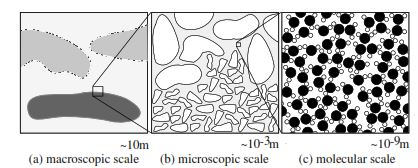
\includegraphics[scale=1]{Imagenes/tipos-de-escalas-peter-bastian}
	%\caption{Diferentes escalas de un medio poroso tomado de la tesis de peter bastian "Numerical Computation of
	%	Multiphase Flows in Porous Media"}
	%\label{escalas-de-medios-porosos.}
%\end{figure}


Peter bastian en su tesis también menciona al realizarse ampliaciones a los suelos a nivel microscópico  se pueden observar espacios vacíos entre sus poros, los cuales pueden llenarse de agua \parencite{Spalding1981}.  Las propiedades de un fluido como la viscosidad, la densidad, el coeficiente de difusión binaria y la miscibilidad, están dadas a escala molecular por propiedades individuales de las moléculas. En la escala microscópica, la configuración del espacio vacío influye en el comportamiento del flujo a través de propiedades como la tortuosidad de los canales de flujo o la distribución del tamaño de los poros, mientras que en la escala macroscópica las inhomogeneidades a gran escala desempeñan un papel importante. Por tanto  el flujo de un fluido newtoniano simple en el espacio vacío de un medio poroso se describe a nivel microscópico mediante el sistema de ecuaciones de Navier-Stokes.

























\section {Estudios Realizados en Colombia}

En el país se han aplicado muchos conceptos matemático a situaciones reales que permiten afianzar los conocimientos en diferentes áreas como ingenierías , un área de la ciencia que ha destacado por la ocupación de métodos numéricos para la solución de problemas ambientales es la hidrología . Es interesante como   \parencite{betancur2009modelacion}  en su artículo realizan un exhaustivo análisis acerca de cómo la modelación numérica puede ser utilizada para fases de exploración hidrogeológica  pues las técnicas de modelación numérica computacional se comportan como una herramienta que permite la interpretación de información y el entendimiento de los sistemas hidrogeológicos estudiados. La modelación numérica enfocada a la dinámica de un fluido subterráneo en un acuífero del bajo cauca antioqueño permitió según la investigación desarrollada y expuesta en el artículo que se elaborara un modelo conceptual de sistema acuífero del Bajo Cauca Antioqueño
permitiendo simular escenarios hipotéticos evaluando con esto posibles respuestas del sistema. \\

En el artículo también se dan datos importantes que permiten dimensionar el alcance que tienen los modelos matemáticos planteados desde hace siglos, las aguas subterráneas se estudian a partir de las leyes de la hidrodinámica, donde conceptos como la porosidad, permeabilidad,  transmisividad y coeficiente de almacenamiento  obtienen relevancia. La ley de Darcy fue clave en la investigación en este artículo. Al tomar como punto de partida un sistema de ecuaciones diferenciales parciales que rigen el flujo de agua subterránea, se logró la obtención de un modelo numérico que representa la hidrodinámica del medio acuífero considerado.  Se planteó que la combinación matemática entre las ecuaciones de balance de masas y la ley de Darcy,  dan lugar a la ecuación que describe el flujo de agua subterránea. 
\begin{equation}
	\frac{\partial }{\partial x}\left ( K_{x}\frac{\partial h}{\partial x} \right ) +\frac{\partial }{\partial y}\left ( K_{y}\frac{\partial h}{\partial x} \right ) +\frac{\partial }{\partial z}\left ( K_{z}\frac{\partial h}{\partial x} \right ) = S_{s}\frac{\partial h}{\partial x}
	\label{Estudioslocales1}    
\end{equation}

En la ecuación \eqref{Estudioslocales1} se distingue que $K_{i}$ representa la conductividad hidráulica del medio en la dirección $i$  $\frac{\partial h}{\partial I}$ que a su vez  representa el gradiente hidráulico $S_{s}$.\\

Por otra parte, \parencite{velez2004metodos} ocupa métodos analíticos, numéricos y empíricos para aproximar de manera continua la recarga que tiene un acuífero. Entre las técnicas que utiliza están las técnicas de Darcy las cuales según su investigación le permiten encontrar valores de cabezas hidráulicas a partir de las ecuaciones de Richards, y 
Boussines,  en las zonas no saturadas. Teniendo como dato experimental la conductividad  hidráulica, coeficiente de almacenamiento del acuífero y contenido de humedad. Y resolver dichas ecuaciones mediante el uso de técnicas analíticas o modelos numéricos computacionales.\\

Una equivalencia de la  ecuación de Richards es 
\begin{equation}
	\frac{\partial \theta }{\partial t} = \frac{\partial }{\partial z} k (\theta)\frac{\partial h }{\partial z} - R_{w}
	\label{Estudioslocales2}    
\end{equation}

Donde :

$\frac{\partial \theta }{\partial t}$  =  es la variación de la humedad con el tiempo.  

$\frac{\partial h }{\partial z}$  =  es la variación de q con la distancia recorrida.

$R_{w}$ = es la extracción de agua por las raíces \\

La ecuación de Boussinesq en una o más dimensiones se puede escribir como :
\begin{equation}
	\frac{S}{T} \frac{\partial h}{\partial t} = k\frac{\partial }{\partial z}\left ( \frac{\partial h }{\partial z} \right ) = k\nabla^2h
	\label{estudioslocales3}
\end{equation}

La ecuación \eqref{estudioslocales3} es para una sola dirección. 

\begin{equation}
	\frac{S}{T} \frac{\partial h}{\partial t} =\frac{\partial }{\partial z}\left ( \tau\frac{\partial h }{\partial z}  \right ) + \frac{\partial }{\partial y}\left ( \tau\frac{\partial h }{\partial y}  \right )
	\label{estudioslocales4}
\end{equation}

La ecuación \eqref{estudioslocales4} es para dos direcciones.\\

Los modelos numéricos que buscan dar solución a la ecuación de Richards intentan representar el flujo de agua, sin embargo muy a menudo se tienen en cuenta muchas suposiciones con el fin de reducir el trabajo computacional. Por tanto la investigación plasmada en este artículo plantea que la complejidad de los modelos numéricos para la zona no saturada radica en la obtención del valor de conductividad hidráulica, pues esta no es constante y varía solo con la textura y estructura del suelo.  Es decir que lo complejo de las limitaciones que posee un modelo numérico computacional no son las debidas a los dispositivos del cálculo, sino los propios a la formulación de los modelos conceptuales del proceso que ocurre en el campo y la definición de las condiciones iniciales del contorno.\\


Por su parte \parencite{garcia2017modelacion}  en su tesis realizó un estudio experimental de modelación matematica del flujo en una zona no saturada en una parcerla situada en Cali- valle del Cauca, Colombia. También expresa que la simulación del flujo de agua se se realizó  con el código HYDRUS-1D. El cual es un programa numérico se basa en van Genuchten para simular el flujo y usa el método de Penman-Moteith para el cálculo de la evapotranspiración de las plantas.\\

En la tesis se menciona que la zona no saturada es una parte fundamental en el ciclo hidrológico en los aspectos relativos a infiltración, evaporación, toma de agua por las raíces de la planta y recarga de agua subterránea de cualquier suelo. Por lo que HYDRUS-1D, sirve extremadamente bien para modelar y simular  el flujo de agua, calor y solutos a través de medios porosos con condiciones de saturación variables. El programa resuelve mediante el método de diferencias finitas la ecuación de Richards modificada en el flujo de agua en medio saturado y no saturado.  Entendiéndose que la ecuación de flujo en medio no saturado es un  concepto ligado al  flujo de agua unidimensional en un medio poroso no deformable y parcialmente saturado el cual  se describe con la ecuación de Richards modificada \eqref{estudioslocales5} . Esta formulación supone que la presión del aire permanece constante sin afectar al flujo de la fase líquida y, además, no considera el efecto de los gradientes térmicos, eléctricos y de salinidad en el movimiento del agua.

\begin{equation}
	\frac{\partial \theta }{\partial t} =  \frac{\partial }{\partial x}\left [ K\left ( \frac{\partial h}{\partial x} \right )+\cos\alpha  \right ]-s
	\label{estudioslocales5}    
\end{equation}

Donde, $h$, es la presión matricial del agua $[L]; \theta$, es el contenido de agua volumétrico [L3L -3 ]; t, es el tiempo $[T]; x$, es la coordenada espacial vertical [L]; S, es el término fuente-sumidero [L3L - 3T -1 ], que en el caso de suelos cultivados representa la cuantía de la extracción de agua por las raíces de las plantas;$\alpha$ es el ángulo entre la dirección del flujo y la vertical ($\alpha $ = 00 para flujo vertical); $K$, es la función conductividad hidráulica no saturada [LT-1 ] definida como:

\begin{equation}
	k(k,x)=K_{s}(x)K_{r}(h,x)
	\label{estudioslocales6}    
\end{equation}

Teniendo en la ecuación \eqref{estudioslocales6} que $K_{r}$, es la conductividad hidráulica relativa $[-]$ y $K$ la conductividad hidráulica saturada.$[LT^{1}]$.\\

Es muy importante mencionar que HYDRUS-1D usa el método de diferencias finitas para proceder a la discretización de la ecuación de Richards, presentada en la expresión \eqref{estudioslocales5} por lo que los datos obtenidos en la investigación son muy representativos del terreno analizado en Cali, Valle del Cauca. Dejando ver que se usó una metodología enteramente numérica ocupado el modelo propuesto por van Genuchten y Mualem  para analizar el movimiento del agua .Por otra parte,  la evapotranspiración fue   calculada a partir del método de Penman-Moteith, todos ellos incluidos en HYDRUS. Es interesante también que en la investigación  la evapotranspiración fue  obtenida a través del propio programa a partir de las condiciones de contorno de la superficie introducidas, constituyendo una limitación más para la obtención de buenos resultados.\\